%\documentclass[ignorenonframetext,11pt]{beamer}
\usepackage[english]{babel}
\usepackage[utf8]{inputenc}
\usepackage{lmodern}
\usepackage{amsmath,amssymb,amsfonts}


% only presentation 
\mode<presentation>
{
  \usetheme{default}
  \setbeamercovered{transparent}
  \usefonttheme{structurebold}
  \setbeamertemplate{theorems}[numbered]
  \usepackage{amscd}
}

\usepackage{multicol}
\usepackage{enumerate}
\usepackage{color}
\usepackage{stmaryrd}
\usepackage{lmodern}



\title{DUNE PDELab Tutorial C++ Refresher}
\author{Olaf Ippisch}
\institute[]
{
  Institut für Mathematik, TU Clausthal\\
  Erzstr. 1, D-38678 Clausthal-Zellerfeld \\[6pt]
}
\date[\today]{\today}

% logo nach oben
\mode<presentation>
{
% No navigation symbols and no lower logo
\setbeamertemplate{sidebar right}{}

% logo
\newsavebox{\logobox}
\sbox{\logobox}{%
    \hskip\paperwidth%
    \rlap{%
      % putting the logo should not change the vertical possition
      \vbox to 0pt{%
        \vskip-\paperheight%
        \vskip0.35cm%
        \llap{\insertlogo\hskip0.1cm}%
        % avoid overfull \vbox messages
        \vss%
      }%
    }%
}

\addtobeamertemplate{footline}{}{%
    \usebox{\logobox}%
}
}

%%%%%%%%%%%%%%%%%%%%%%%%%%%%%%%%%%%%%%%%%%%%%%%%%%%%%%%%%%%%%%%%%%%%%%%%%%%%%%%%
%%%%%%%%%%%%%%%%%%%%%%%%%%%%%%%%%%%%%%%%%%%%%%%%%%%%%%%%%%%%%%%%%%%%%%%%%%%%%%%%
%
% now comes the individual stuff lecture by lecture
%
%%%%%%%%%%%%%%%%%%%%%%%%%%%%%%%%%%%%%%%%%%%%%%%%%%%%%%%%%%%%%%%%%%%%%%%%%%%%%%%%
%%%%%%%%%%%%%%%%%%%%%%%%%%%%%%%%%%%%%%%%%%%%%%%%%%%%%%%%%%%%%%%%%%%%%%%%%%%%%%%%

\begin{document}

\begin{onlyenv}<article>
\maketitle
\end{onlyenv}

\frame{\titlepage}

%%%%%%%%%%%%%%%%%%%%%%%%%%%%%%%%%%%%%%%%%%%%%%%%%%%%%%%%%%%%%%%%%%%%%%%%%%%%%%%%
%%%%%%%%%%%%%%%%%%%%%%%%%%%%%%%%%%%%%%%%%%%%%%%%%%%%%%%%%%%%%%%%%%%%%%%%%%%%%%%%

\begin{frame}
  \frametitle{Goals of this introduction}
  A number of advanced C++ features is required to use DUNE or makes
  its usage much easier. Some of them were introduced in the last
  C++ language-standards  C++11, C++14 and C++17. We will specifically look at:
  \begin{itemize}
  \item Compiling Programs on Linux-based systems
  \item Object-Oriented Programming
  \item Namespaces
  \item Automatic type deduction
  \item Templates
  \item Containers of the C++ standard library
  \item Range-based for loops
  \item Lambda functions
  \end{itemize}
\end{frame}

\section{Compiling Programs on Linux}
\begin{frame}[fragile]
  \frametitle<presentation>{Compiling Programs}
  On Linux-based systems, the (GNU-)C++ compiler is called \inline!g++!. In order to compile a program from the source file \inline!main.cc! and create an executable called \inline!myprogram! you run it like this:
  \begin{lstlisting}
  g++ -o myprogram main.cc
  \end{lstlisting}
With \lstinline!g++! the C++14 standard is the default since version 6.1. If you want to use C++17 or if you use the Intel compiler or \lstinline!clang!, you can set the standard with the option \lstinline!-std=c++14! or \lstinline!-std=c++17! (on Windows systems the options may be different), e.g.
  \begin{lstlisting}
  g++ -std=c++17 -o myprogram main.cc
  \end{lstlisting}

If your program was compiled successfully (without error messages), you run it with:
  \begin{lstlisting}
  ./myprogram
  \end{lstlisting}
and get for example the output
  \begin{lstlisting}
  Hello, world!
  \end{lstlisting}
\end{frame}

\begin{frame}[fragile]
  \frametitle<presentation>{Compiling Programs}
  For more complex software projects usually so-called makefiles are provided. A makefile ensures that all relevant source files for the project are compiled, when the command \inline!make! is executed:
  \begin{lstlisting}
  make
  \end{lstlisting}
  If you build the project after changing only some source files, only these files are recompiled, which can speed up the process considerably.
  
  For DUNE the makefiles are generated by a tool called \inline!cmake!.
\end{frame}

\section{Object-Oriented Programming}

\begin{frame}
\frametitle<presentation>{Object-Oriented Programming}
The basic idea of object-oriented programming is to define components with a certain functionality. These components combine both the methods which are needed to provide and control the functionality as well as the relevant data. Different components are connected via interfaces. The same interface is used for specialised components providing the same general functionality.

This approach has several advantages:
\begin{itemize}
\item Different components can be developed separately.
\item If improved versions of a component become available, they can be used without major changes to the program code.
\item Several realisations of the same component can be used easily.
\end{itemize}

This is also used in the real world, e.g. the tires of a car, the socket of a CPU, the USB interface of computers, printers, mobile phones \dots
\end{frame}

\begin{frame}
\frametitle{Object-oriented Programming in C++}
In C++ this idea is realised by classes and objects. Classes describe the functionality and structure of a component. Realisations of this blueprint are called objects. 

Let us use a two-dimensional vector as example:
\begin{itemize}
\item The vector consists of two components.
\item The necessary operations are length (norm), sum of two vectors, multiplication of a vector with a scalar,\dots.
\item Initialization: Create a vector with a defined state.
\end{itemize}\ \\
$(1,3)$ and $(5,0)$ are different vectors, but they share the same structure.\\
\pause
\begin{block}{$\Rightarrow$ C++ language concept}
\inline!class! describes semantics of similar objects (vectors, function spaces, linear solvers,\dots).
\end{block}
\end{frame}

\begin{frame}[fragile]
  \frametitle{Classes}
  \begin{lstlisting}
class Point2D {
public:
  Point2D(double x_, double y_)
    : x(x_), y(y_)
  {}

  double norm() const {
    return sqrt(x*x + y*y);
  }

  void add(const Point2D &p) {
    x += p.x;
    y += p.y;
  }

private:
  double x, y;
};
  \end{lstlisting}
\end{frame}

\begin{frame}[fragile]
  \frametitle{Using C++ Objects}
 Classes define a new data type. 
\begin{itemize}
  \item Variables of \inline!class! type are called objects and can be used like other types (\inline!int!, \inline!double!, \dots):
    \begin{lstlisting}
      // calls constructor, initialises data
      Point2D p = Point2D(3.0,4.1); 
    \end{lstlisting}
  \item The member variables and functions of an \emph{object} are accessed over the variable name followed by a dot and the name of the variable/function:
    \begin{lstlisting}
      std::cout << p.norm() << std::endl;
    \end{lstlisting}
  \item Objects of a \inline!class! can be used like ordinary variables:
    \begin{lstlisting}
      Point2D p2 = p; // create a copy of p
      p.add(p2);
    \end{lstlisting}
  \end{itemize}
\end{frame}

\begin{frame}[fragile]
  \frametitle{Encapsulation}
  \begin{itemize}
  \item Data members and methods of a \inline!class! can be either \inline!public! (accessible from outside the \inline!class!) or \inline!private! (accessible only from methods of the same \inline!class!).
  \item If you try to access a \inline!private! member from outside the class, you get a compiler error:
    \begin{lstlisting}
      std::cout << p.x << std::endl; // compiler error!
    \end{lstlisting}
  \item It is advisable to make the data members of a \inline!class! private. This is called \emph{encapsulation} and facilitates a later change of the way the data is stored, which can often greatly improve performance. 
  \end{itemize}
\end{frame}

\section{Namespaces}

\begin{frame}[fragile]
  \frametitle<presentation>{Namespaces}
  \begin{itemize}
  \item Let us assume you want to use two existing libraries with the header files \inline!linear_solver.h! and \inline!nonlinear_solver.h!. 
  \item Both define a function \inline!solve_problem()!. 
  \item The compiler cannot distinguish between them!
  \item How can you use both libraries without name conflicts? 
  \end{itemize}
  
\end{frame}

\begin{frame}[fragile]
  \frametitle<presentation> {Namespaces}
  C++ uses namespaces, which allows an easy resolution of this problem:
\begin{lstlisting}
  namespace linsolv {
    #include<linear_solver.h>
  }
  namespace nonlinsolv {
    #include<nonlinear_solver.h>
  }
  int main() {
    linsolv::solve_problem();
    nonlinsolv::solve_problem();
  }
\end{lstlisting}
Each \inline!class! automatically defines a namespace with the name of the \inline!class! which contains its data members and functions.
\end{frame}

\begin{frame}[fragile]
  \frametitle{Builtin Namespace \texttt{std}}
  \begin{itemize}
  \item C++ also contains a library of useful functions and classes the so called standard library. 
  \item Beginners often write 
  \begin{lstlisting}
  using namespace std;
  \end{lstlisting}
at the top of their program, which imports all functions of the standard library into the global namespace.
  \item You should \emph{NEVER} do this as it can lead to name conflicts and reduces flexibility in further development!
  \end{itemize}
  
\end{frame}

\begin{frame}[fragile]
  \frametitle<presentation>{Builtin Namespace \texttt{std}}
Just write the namespace \inline!std::! in front of the functions and types instead:
  \begin{lstlisting}
    #include <iostream>
    #include <cmath>

    int main()
    {
      double v = 2.0;
      double s = sqrt(v);
      std::cout << "The square root of " << v
                << " is " << s << std::endl;
    }
  \end{lstlisting}
  If you use the auto-completion features of modern editors, this is not much typing overhead and much less work than rewriting your code later.
\end{frame}

\section{Automatic Type Deduction}

\begin{frame}
\frametitle<presentation>{Automatic Type Deduction}

Since C++11 the type needed for a variable can be detected automatically if it can be deduced from the initialization of the variable. This is indicated with the keyword \inline!auto!.

\lstinputlisting{auto.cc}

\end{frame}

\begin{frame}[fragile]
\frametitle{\texttt{auto}: Advantages}

\begin{itemize}
\item Using \inline!auto! instead of manually writing the exact type (e.g.~\inline!int!) has a lot of advantages (at the expense of a bit of detailed control):
\begin{itemize}
\item If you create a variable with \inline!auto!, it will always be initialized with an defined value, which avoids a whole class of very subtle bugs.
\item If you write \inline!auto!, the compiler can choose the right type, reducing the risk of errors.
\item When using advanced libraries like DUNE, the types of variables can become very complicated, making it difficult to read code that spells out those types.
\end{itemize}
\item Only since C++14 it is possible to use \inline!auto! in function definitions and declarations.
\end{itemize}

\end{frame}

\begin{frame}
\frametitle{\texttt{auto} and literals}

For type deduction with \inline!auto! the usual rules for C++ literals apply:

\lstinputlisting{auto3.cc}

\end{frame}

\begin{frame}[fragile]
  \frametitle{References}
  \begin{itemize}
  \item If variables are passed to a function in C++, by default a copy of the variable is generated. 
  \item References are an alternative, which only generates a new name for the same data. 
  \item References are generated by adding a \inline!&! between the data type and the variable name, e.g. \inline!int &blub=blob! or \inline!int f(int &a)!. 
  \item You can only generate references to existing variables not to literals!
  \end{itemize}
  
\end{frame}

\begin{frame}[fragile]
  \frametitle<presentation>{\texttt{auto} and References}
  \begin{itemize}
  \item If you want to make a variable a reference with automatic type deduction write \inline!auto &! instead of \inline!auto!:
  \end{itemize}

  \begin{lstlisting}
    /* Copying */
    auto i = 4;
    auto j = i;  // i = 4, j = 4, j is a copy
    i += 1;      // i = 5, j = 4
    j -= 1;      // i = 5, j = 3
    j  = i;      // i = 5, j = 5

    /* Referencing */
    auto &k = i; // i = 5, k = 5, k is a reference to i
    i  = 2;      // i = 2, j = 5, k = 2
    i += 1;      // i = 3, j = 5, k = 3
    k  = 8;      // i = 8, j = 5, k = 8
  \end{lstlisting}
\end{frame}


\section{Templates}

%-----------------------------------------------------------------------------

\begin{frame}[fragile]
\frametitle<presentation>{Generic Programming}


\begin{itemize}%[<+->]
\item Often the same algorithms are needed for different data types.
\item Without generic programming one has to write the same function for all data types, which is tedious and error-prone, e.g.
\end{itemize}
\vspace*{-10mm}
\begin{multicols}{2}
    \begin{lstlisting}
      int Square(int x)
      {
        return(x*x);
      }

      float Square(float x)
      {
        return(x*x);
      }
    \end{lstlisting}

    \begin{lstlisting}
      long Square(long x)
      {
        return(x*x);
      }

      double Square(double x)
      {
        return(x*x);
      }      
    \end{lstlisting}
\end{multicols}
\vskip-7mm
\begin{itemize}
\item Generic programming allows to write the algorithm once and parametrise it with the
data type.
\end{itemize}

\end{frame}

%-----------------------------------------------------------------------------

\begin{frame}[fragile]
\frametitle{Template functions}
\begin{itemize}%[<+->]
\item A function template starts with the keyword \inline|template| and a list of one or more template arguments
in angle brackets separated by commas:
\begin{lstlisting}
template<typename T>
T Square(T a)
{
    return(a*a);
}
\end{lstlisting}
\item If a template is used, the compiler can automatically generate the function from the function template according to the function arguments (as with overloading the return type is not relevant).
 \item The template arguments can also be specified explicitly:
 \begin{lstlisting}
     std::cout << Square<int>(4) << std::endl;
 \end{lstlisting}
 \item The argument types must fit the declaration
\end{itemize}
\end{frame}

%-----------------------------------------------------------------------------

\begin{frame}[fragile]
\frametitle{Example: Unary Template Function}
\begin{lstlisting}
#include<cmath>
#include<iostream>

template<typename T>
T Square(T a)
{
    return(a*a);
}

int main()
{
    std::cout << Square<int>(4) << std::endl;
    std::cout << Square<double>(M_PI) << std::endl;
    std::cout << Square(3.14) << std::endl;
}
\end{lstlisting}
\end{frame}

%-----------------------------------------------------------------------------

\begin{frame}[fragile]
\frametitle{Example: Binary Template Function}
\begin{lstlisting}
#include<cmath>
#include<iostream>

template<class U>
const U &max(const U &a, const U &b) {
 if (a>b)
     return(a);
 else
     return(b);
}

int main()
{
 std::cout << max(1,4) << std::endl;
 std::cout << max(3.14,7.) << std::endl;
 std::cout << max(6.1,4) << std::endl; // compiler error
 std::cout << max<double>(6.1,4) << std::endl; // correct
 std::cout << max<int>(6.1,4) << std::endl;    // warning
}
\end{lstlisting}
\end{frame}

%-----------------------------------------------------------------------------

\begin{frame}[fragile]
\frametitle{Useful predefined template functions}
The C++ standard library already provides some useful template functions:
\begin{itemize}%[<+->]
\item \inline!const T& std::min(const T& a, const T& b)! \\
  minimum of a and b\\
  \begin{lstlisting}
    auto c = std::min(a,b);
  \end{lstlisting}
\item \inline!const T& std::max(const T& a, const T& b)! \\
  maximum of a and b\\
  \begin{lstlisting}
    auto c = std::max(a,b);
  \end{lstlisting}
\item \inline!void std::swap(T& a, T& b)! \\
  swap a and b\\
  \begin{lstlisting}
    std::swap(a,b);
  \end{lstlisting}
\end{itemize}
\end{frame}


%-----------------------------------------------------------------------------

\begin{frame}[fragile]
\frametitle{Class Templates, Non-type Template arguments, \\ default arguments}
\begin{lstlisting}
template<typename T, int dimension = 3>
class NumericalSolver
{
    ...
  protected:
    T variable;
};
\end{lstlisting}
\begin{itemize}%[<+->]
\item Template arguments can be used in class declarations.
\item Not only types, but also integer values can be used as template arguments. The values used in the template instantiation have to be compile time constants.
\item If templates are used in a class definition, the last template arguments can have default values.
\item The name of a class is the class name plus the template parameters
\end{itemize}

\end{frame}

%-----------------------------------------------------------------------------

\begin{frame}[fragile]
\frametitle{Inheritance from Class Templates}
\begin{lstlisting}
template<typename T>
class MyNumericalSolver : public NumericalSolver<T,3>
{
    T myVariable;
  public:
    MyNumericalSolver(T val) : NumericalSolver<T,3>(),
                               myVariable(val)
    {
      std::cout << NumericalSolver<T,3>::variable
                << std::endl;
    };
};
\end{lstlisting}
\begin{itemize}%[<+->]
\item If a class is derived from a template class, the template arguments have to be given as
part of the base class name.
\item the same is true for the call of base class constructors and the prefixing
of base class members and methods.
\end{itemize}

\end{frame}


%-----------------------------------------------------------------------------

\begin{frame}[fragile]
\frametitle{Using Members of a Template Base Class}
\begin{lstlisting}
template<typename T>
class MyNumericalSolver : public NumericalSolver<T,3>
{
    T myVariable;
  public:
    MyNumericalSolver(T val) : NumericalSolver<T,3>(),
                               myVariable(val)
    {
        this->variable=val;
    };
};
\end{lstlisting}
\begin{itemize}
\item The members of a template base class are often not automatically resolved correctly
\item To avoid problems, it is (as a rule of thumb) helpful to always prefix
base class members (methods as well as variables) with \inline!this->!
\end{itemize}

\end{frame}


%-----------------------------------------------------------------------------

\begin{frame}[fragile]
\frametitle{Template Compilation}
\begin{itemize}
\item If templates are not used and therefore are not instantiated, the template code is only
checked for crude syntax errors (e.g.~missing semicolons) by the compiler.
\item The test, if all function calls are valid, is conducted when a template is instantiated.
Errors like missing functions are only detected then. The error messages can be rather strange.
\item As the code is only created at the template instantiation, the compiler has to know at this
time the whole function definition not only its declaration.
\item The usual subdivision into header and source files is therefore not possible for templates.
\end{itemize}
\end{frame}

%-----------------------------------------------------------------------------

\begin{frame}[fragile]
\frametitle<presentation>{Template Compilation}
\begin{itemize}
\item To save computation time and memory, only class functions which are really called are generated.
\item Thus
class templates can also be instantiated for types which do not support all necessary operations as long
as the methods where they are needed are never called.
\item If template classes have long argument lists, typedefs are helpful:
\begin{lstlisting}
typedef Point2D P;
auto coord = P(8,1); // Now P means the same as Point2D
\end{lstlisting}

\end{itemize}
\end{frame}

\begin{frame}[fragile]
\frametitle{Template Aliases}
\begin{lstlisting}
template <typname U>    // create partially defined templates 
using VectorSpace = Dune::PDELab::Backend::Vector<GFS,U>::type;

int main()
{
  using int32 = int;                  // rename ordinary types
  using Vector = 
        typename Dune::PDELab::Backend::Vector<GFS,double>::type;
  auto v = Vector(gfs); // Save lots of typing...
  using Function = void (*)(double);  // function types
  VectorSpace<float> blub;
}
\end{lstlisting}


\begin{itemize}
\item An alternative method to define abbreviations for long type names is called ``template aliasing''.
\item Also partial template aliasing is possible fixing some of the template arguments.
\end{itemize}

\end{frame}


%-----------------------------------------------------------------------------

\begin{frame}[fragile]
\frametitle{Keyword \texttt{typename}}
\begin{lstlisting}
template<typename T, int dimension = 3>
class NumericalSolver : public T::ClassType
{
    ...
    typename T::SubType doSomething(
                          typename T::OtherSubType argument);
  private:
    typename T::SubType variable;
}
\end{lstlisting}
\begin{itemize}%[<+->]
\item In C++ by default a member of a class template is assumed not to be a type but
a (static) variable.
\item The \inline!typename! keyword is needed to
indicate that the member of a class (which is given as or depends on a template
parameter) is a type.
\item It is only needed/allowed inside a template.
\item It is not used in a list of base class specifications or in a list of member initializers
in a constructor definition
\end{itemize}

\end{frame}


%-----------------------------------------------------------------------------

\begin{frame}[fragile]
\frametitle{Keyword \texttt{.template}}
\begin{lstlisting}
class A
{
  public:
    template<class T> T doSomething() { };
};

template<class U> void doSomethingElse(U variable)
{
    char result = variable.template doSomething<char>();
}

template<class U,typename V> V doSomethingMore(U *variable)
{
    return variable->template doSomething<V>();
}
\end{lstlisting}
\begin{itemize}%[<+->]
\item C++ assumes by default that every \inline!<! character following an object is the start of a comparison.
\item The keyword \inline!template! in front of such a method name indicates that
an explicit template parameter follows.
\end{itemize}

\end{frame}


%-----------------------------------------------------------------------------

\section{The C++ Standard Library}

%-----------------------------------------------------------------------------

\begin{frame}
\frametitle<presentation>{The C++ Standard Library}
The standard library (sometimes called STL for Standard Template Library) is
\begin{itemize}%[<+->]
\item a collection of useful template functions and classes.
\item available for all modern C++ compilers.
\item optimised for efficiency.
\item a lot safer than using plain C libraries and data structures.
\end{itemize}
\end{frame}

%-----------------------------------------------------------------------------

\begin{frame}
\frametitle{STL-Containers}

\begin{itemize}
\item Data representation is often crucial for the efficiency of algorithms
\item The STL defines containers and algorithms to use them.
\item Containers are used to manage a collection of elements
\item Iterators provide a common interface to traverse the elements of a container
\item There is a wide variety of containers optimised for different purposes:
\begin{center}
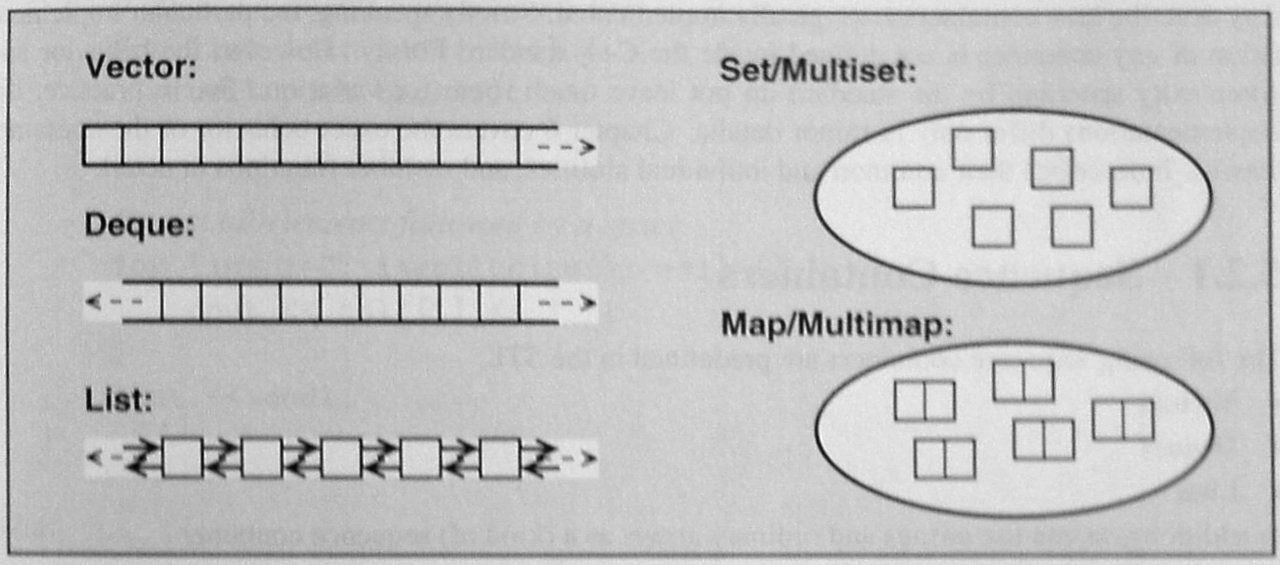
\includegraphics[width=9cm]{containers.jpg}

figure from: \cite{josuttis99:stl}
\end{center}
\end{itemize}

\end{frame}

%-----------------------------------------------------------------------------


\begin{frame}
  \frametitle{Library Example: dynamic array}
  The STL contains a dynamic array called \inline!std::vector! which is a lot better than its plain
  C counterpart:
  \begin{itemize}
  \item It automatically frees the memory when you don't need it anymore, avoiding memory leaks.
  \item It knows about its size, so you don't have to remember it.
  \item It can automatically resize itself if you need a larger vector.
  \item It is a template: You specify the type of object to store inside of it.
  \item It is fast.
  \end{itemize}
\end{frame}


% \begin{frame}
% \frametitle{Vec}
% Sequence Containers are ordered collections, where each element has a certain position.
% \begin{description}%[<+->]
% \item[Vector] is a dynamic array of elements.
% \begin{itemize}
% \item elements can be accessed directly with an index (random access).
% \item appending and removing at the end is fast.
% \end{itemize}
% % \item[Deque], the ``double-ended'' queue, is a dynamic array.
% % \begin{itemize}
% % \item can grow in both directions.
% % \item elements can be accessed directly with an index, however, if elements are inserted at the front, the index of a certain element might change.
% % \item appending and removing elements at the end and the beginning is fast.
% % \end{itemize}
% \end{description}
% \end{frame}

%-----------------------------------------------------------------------------

\begin{frame}[fragile]
\frametitle{Vector Example}
The following example shows how to use a \inline!std::vector!:
\begin{lstlisting}
#include <iostream>
#include <vector>

int main()
{
    auto b = std::vector<double>(7); // a vector for 7 doubles
    std::cout << b.size() << std::endl; // output the size
    for (int i = 0; i < b.size() ; ++i)
        b[i] = i*0.1; // assign some data
    auto c = b; // create a copy, automatically copying all data
    c.resize(15); // Make c bigger
    std::cout << b.size() << std::endl; // still 7
    b.push_back(3.8); // make b larger and append the value 3.8
}
\end{lstlisting}
\end{frame}

\begin{frame}
\frametitle{Iterators}
\begin{itemize}
\item An essential part of the Container concept is a generalised scheme to iterate over all elements stored in a container, which is independent of the container type using so-called iterators.
\item The syntax of iterator usage is derived from the usage of pointers in ordinary C.
\item Each container has a method \inline!begin()!, which returns an iterator pointing to the first member of the container.
\item The iterator has the data type \inline!containerclass::iterator! (but you don't need to know this if you use auto).
\item If you call the increment operator \inline!++! of the iterator, it will afterwards point to the next element.
\item You can check if you reached the end of the container by comparing the iterator to \inline!container.end()!.
\end{itemize}
\end{frame}

\begin{frame}
\frametitle<presentation>{Iterators}
\begin{itemize}
\item To access the element to which the iterator points, you have to dereference it, e.g. \inline!*it!
\item If the element of the container is an object of a class, you can also use the operator \inline!it->! to access data members or functions of the class.
\end{itemize}
\lstinputlisting{iterator.cc}
\end{frame}

\section{Range-based for Loops}

\begin{frame}[fragile]
  \frametitle<presentation>{Range-based \texttt{for} Loops}
  With range-based \inline!for! loops the same operation (iterating over a whole container) can be written much simpler:
  \begin{lstlisting}
    auto vec = std::vector<double>(8);
    for (auto d : vec)
      std::cout << d << std::endl; // prints all entries of vec
  \end{lstlisting}
  \begin{itemize}
  \item Works for C arrays and all STL containers.
  \item Also important for using DUNE!
  \item Careful: what you get in a range-based \inline!for!-loop is not an iterator. You don't have to dereference it. You can directly use it to access the content.
  \end{itemize}
\end{frame}

\begin{frame}[fragile]
  \frametitle<presentation>{Range-based \texttt{for} Loops}

  You can get either a copy or a reference (if you write \inline!auto &!) of the element currently accessed.

  \begin{lstlisting}
    #include<iostream>
    #include<vector>

    int main()
    {
      std::vector<double> x(5);
      int i=0;
      for (auto &y : x) {       // with reference
        y = i * 1.2;            // can be changed
        ++i;
      }
      for (auto y : x) {        // with copy
        y *= y;                 // original container unchanged
        std::cout << y << std::endl;
      }
    }
  \end{lstlisting}

\end{frame}

\section{Type Deduction for Function Argumetns}

\begin{frame}[fragile]
\frametitle{Decltype}
\begin{itemize}
\item \lstinline!decltype! determines the result type of an expression (not the result value). It can be used to make matching variables.
\begin{lstlisting}
int a,b;
decltype(a+b) c;
\end{lstlisting}
\item Together with template aliasing it can 
be used to store types:
\inline!using type = decltype(expression)! 
\item Difference to \inline!auto!: Does not create a variable of the same type but stores the type, also preserves references.
\item Good if you want to store the result of a function call in a container.
\end{itemize}
\begin{lstlisting}
template<typename Vector>
auto squareroot_values(const Vector& v)
{
  using R = decltype(sqrt(v[0])); // result type of std::sqrt()
  auto result = std::vector<R>();
  for (auto d : v)           // create a vector of square roots
    result.push_back(std::sqrt(d)); 
  return result;
}
\end{lstlisting}

\end{frame}

\begin{frame}[fragile]
\frametitle{Historic: \lstinline!decltype! and return values in C++11}
\begin{itemize}
\item In C++11 \inline!auto! could not be used directly for function definitions or declarations. This is only possible since C++14.
\item The return type of a function could be determined depending on the type of the function arguments with \inline!decltype!
\item \inline!decltype! determines the type of a given operation.
\item In the easiest version, \inline!auto! is used as return type and \inline!-> decltype(op)! is added after the argument list of the function, where \inline!op! is a given operation:
\end{itemize}
\begin{lstlisting}
template<typename T, typename U>
auto add(T t, U u) -> decltype(t + u);
\end{lstlisting}

\end{frame}


\section{Lambda Functions}

\begin{frame}[fragile]
  \frametitle<presentation>{Lambda functions}
  \begin{itemize}
  \item C++11 introduced a simplified possibility to create (mostly temporary) functions, so-called lambda expressions or lambdas.
  \item Example:
\begin{lstlisting}
auto f = [](auto x) -> double 
{
  double y = x;
  return std::sin(y);
};
\end{lstlisting}
\item There is an even shorter version for single expressions (return type auto-deduced):
\begin{lstlisting}
auto f = [](auto x) { return std::sin(x); };
\end{lstlisting}
\item Lambdas can be stored like variables, the type of lambda functions is implementation-defined. Thus \inline!auto! variables have to be used.
  \end{itemize}
\end{frame}

\begin{frame}[fragile]
  \frametitle{Lambda functions: Syntax}
\inline![capture-list](parameter-list) -> return-type { code; }!
\vspace*{1em}
  \begin{itemize}
  \item Lambdas do not have a function name. 
  \item They start with a capture list, determining which variables from the surrounding scope are available inside the lambda
  \item This is followed by a ordinary parameter list and a return (specified similar to \lstinline!decltype!) and finally the code block of the function.
  \item Two types of capture: by value (creates a copy) or by reference (points to the original variable)
  \item Usage: List variable names, add ampersand (\inline!&!) for references
  \item Shortcuts: \inline![=]! capture all variables by value, \inline![&]! capture all variables by reference
  \item Since C++17 it is also possible to capture a variable as constant reference: \inline![&v=std::as_const(v)]!
  \item \structure{Caution:} When using capture by reference, make sure the original variable still exists when calling the lambda function!
  \end{itemize}
\end{frame}

\begin{frame}[fragile]
\frametitle{Lambda functions: Capture Example}
\begin{lstlisting}
auto pi = 3.14;
auto f = [pi](auto x) { return pi * x; };
auto g = [&pi](auto x) { return pi * x; };
f(1); // returns 3.14;
g(1); // returns 3.14;
pi = 3.141;
f(1); // returns 3.14 - value was copied!
g(1); // returns 3.141 - value was referenced!

int call_count = 0;
auto h = [&](auto x) 
{
  ++call_count;
  return pi + x;
}
h(1); // returns 4.141
std::cout << call_count << std::endl; // prints 1
\end{lstlisting}

\end{frame}

\begin{frame}[fragile] \frametitle{Accumulation using
    \inline!for_each!: lambda function}

Lambda functions are very useful for template algorithms as e.g. defined by the standard template library. The \inline!for_each! algorithm applies a function object to each of the elements of a container.

\vspace*{2em}

  \begin{lstlisting}
auto coll = std::vector<double>();
// fill coll with data...
int count = 0;
double sum = 0;
std::for_each(coll.begin(),coll.end(),
              [&](auto x){ ++count; sum += x; } );
std::cout << sum / count << std::endl;
  \end{lstlisting}
\end{frame}



\section{References}

\begin{frame} \frametitle<presentation>{Further Reading}

\begin{thebibliography}{Vandervoorde and Josuttis(2003)}

\bibitem[Stroustrup (2014)]{stroustrup13:cpp_programming}
Bjarne Stroustrup.
\newblock \emph{Programming: Principles and Practice Using C++}.
\newblock Addison Wesley, 2014.

\bibitem[Stroustrup(2013)]{stroustrup13:cpp_language}
Bjarne Stroustrup.
\newblock \emph{The C++ Programming Language}.
\newblock Addison Wesley, 2013.

\bibitem[cppreference.comm]{cppreference}
The cppreference community.
\newblock \emph{The community C++ reference web site.}
\newblock \alert<2>{\url{http://cppreference.com}}.

\end{thebibliography}
\end{frame}

\end{document}

